\documentclass[12pt,a4paper]{article}
\usepackage[utf8]{inputenc}
\usepackage[T1]{fontenc}
\usepackage{lmodern}
\usepackage[spanish,es-nodecimaldot]{babel}
\usepackage[a4paper,margin=2.5cm]{geometry}
\usepackage{booktabs}
\usepackage{amsmath}
\usepackage{float}
\usepackage{graphicx}
\usepackage{tabularx}
\usepackage{longtable}
\usepackage{array}
\usepackage{hyperref}
\hypersetup{colorlinks=true,linkcolor=black,urlcolor=blue,pdftitle={Proyecto integrador: clasificacion supervisada sobre Seismic-Bumps}}
\setlength{\LTpre}{0.4em}
\setlength{\LTpost}{0.4em}
\newcolumntype{Y}{>{\raggedright\arraybackslash}X}

\title{Proyecto integrador\\[0.75em]Clasificación supervisada de eventos sísmicos peligrosos en minería subterránea: comparación de árbol de decisión, Naive Bayes, k-NN y regresión logística}
\author{Martinez Mauricio Leonel\\DNI: 45.549.925}
\date{2026}

\begin{document}

\begin{titlepage}
\thispagestyle{empty}
\begin{center}
{\Large\textbf{Universidad Católica de Salta (UCASAL)}}\\[0.4cm]
{\large Facultad de Ingeniería}\\[1.2cm]
{\large\textbf{Materia:} Técnicas avanzadas de análisis de datos}\\[2.2cm]

{\LARGE\bfseries Proyecto integrador}\\[0.7cm]
{\Large\bfseries Clasificación supervisada de eventos sísmicos peligrosos en minería subterránea: comparación de árbol de decisión, Naive Bayes, k-NN y regresión logística}\\[1.2cm]

\rule{0.82\textwidth}{0.4pt}\\[1.2cm]

\begin{tabular}{>{\bfseries}rl}
Estudiante: & Martinez Mauricio Leonel \\
DNI: & 45.549.925 \\[0.35cm]
Docentes: & Cardoso, Alejandra Carolina \\
& Pastrana, Analía Verónica \\
& Talame, María Lorena \\[0.35cm]
Año: & 2026 \\
\end{tabular}

\vfill
{\large Facultad de Ingeniería -- Universidad Católica de Salta}
\end{center}
\end{titlepage}

\begin{abstract}
Este informe final analiza el conjunto \textit{Seismic-Bumps} con el objetivo de comparar cuatro algoritmos de clasificación supervisada para identificar turnos peligrosos en minería subterránea. El archivo utilizado contiene 2584 instancias, 18 atributos predictivos y una variable objetivo binaria, con fuerte desbalance: 170 registros peligrosos frente a 2414 no peligrosos. La metodología se basó en validación cruzada estratificada de 10 particiones en Altair AI Studio y en la lectura conjunta de accuracy, AUC (optimistic), precisión, recall, F1 y matrices de confusión. Los modelos base muestran que la exactitud global puede ocultar una baja detección de la clase peligrosa. La regresión logística base queda como referencia equilibrada por F1 de clase 1, con 32,40\% agregado. Sin embargo, para el objetivo principal del proyecto se selecciona una única configuración final: regresión logística con SMOTE, porque prioriza el recall de la clase peligrosa. Esta variante obtuvo 81,76\% de recall y redujo los falsos negativos a 31, aunque produjo 1219 falsos positivos y una precisión baja de 10,24\%. El resultado es útil como evidencia experimental y como base de decisión, pero no constituye por sí solo un sistema operativo de alerta sin validación temporal, análisis de costos y ajuste explícito del umbral de decisión.
\end{abstract}

\tableofcontents
\newpage

\section{Introducción}
La minería subterránea puede estar expuesta a eventos sísmicos de alta energía que afectan la seguridad de los trabajadores, la infraestructura y la continuidad de las operaciones. En ese contexto, los registros históricos de actividad sísmica y sismoacústica permiten estudiar si el comportamiento observado durante un turno contiene señales útiles para anticipar una situación peligrosa en el turno siguiente. El conjunto \textit{Seismic-Bumps} fue construido precisamente alrededor de ese problema: cada fila resume mediciones de un turno y la clase indica si luego ocurrió un evento de alta energía.

Este proyecto integrador compara cuatro algoritmos de clasificación supervisada: árbol de decisión, Naive Bayes, k-NN y regresión logística. La comparación se realiza sobre un problema binario en el que la clase 0 representa un estado no peligroso y la clase 1 representa un estado peligroso. La evidencia central del informe son las matrices de confusión y las métricas de rendimiento obtenidas en Altair AI Studio mediante validación cruzada estratificada de 10 particiones.

La interpretación no se apoya en una única métrica. El conjunto está fuertemente desbalanceado: la clase peligrosa representa solo el 6,58\% de las instancias. Por lo tanto, un modelo puede alcanzar una exactitud alta clasificando correctamente la mayoría de los casos no peligrosos y, al mismo tiempo, omitir una parte importante de los casos que más interesan. La evaluación se organiza con el patrón claim-evidence-interpretation: primero se formula qué muestra cada resultado, luego se presenta la evidencia numérica y finalmente se interpreta su relevancia para el objetivo del proyecto.

\section{Problema, pregunta y objetivos}
El problema consiste en determinar qué comportamiento presentan distintos algoritmos de clasificación ante un conjunto con clase positiva minoritaria y alto costo potencial de omisión. En este trabajo, un falso negativo significa que un registro peligroso fue clasificado como no peligroso. Desde el punto de vista del objetivo del proyecto, ese error es crítico porque reduce la capacidad de detección de situaciones que podrían requerir supervisión o intervención.

La pregunta de investigación es:
\begin{quote}
¿Qué diferencias presentan un árbol de decisión, Naive Bayes, k-NN y regresión logística en términos de rendimiento global y detección de la clase peligrosa en el conjunto \textit{Seismic-Bumps}, bajo un procedimiento de evaluación común?
\end{quote}

El objetivo general es analizar comparativamente el comportamiento de esos cuatro algoritmos para clasificar la ocurrencia de eventos sísmicos peligrosos. Los objetivos específicos son:
\begin{itemize}
\item describir la estructura del archivo ARFF, sus atributos y la distribución de clases;
\item documentar la preparación de datos sin introducir transformaciones no comprobadas;
\item evaluar los modelos base mediante validación cruzada estratificada;
\item analizar matrices de confusión con filas verdaderas y columnas predichas;
\item comparar accuracy, AUC (optimistic), precisión, recall y F1 de la clase peligrosa;
\item evaluar el efecto de SMOTE aplicado únicamente durante entrenamiento;
\item seleccionar una configuración final coherente con el objetivo de priorizar la detección de la clase peligrosa; y
\item explicitar las limitaciones metodológicas de los resultados obtenidos.
\end{itemize}

\section{Descripción del conjunto de datos}
Se utilizó el archivo local \texttt{seismic-bumps.arff}, correspondiente al conjunto \textit{Seismic-Bumps}. Según el encabezado del ARFF y la descripción del conjunto de datos de Sikora y Wrobel (2010), los datos describen el problema de anticipar eventos sísmicos de alta energía, superiores a $10^4$ J, en una mina de carbón. El archivo contiene 2584 instancias, 18 atributos predictivos y una variable objetivo denominada \texttt{class}. El propio encabezado del ARFF declara que no existen valores faltantes.

\begin{table}[H]
\centering
\caption{Características generales del conjunto de datos.}
\label{tab:dataset-general}
\begin{tabular}{ll}
\toprule
\textbf{Característica} & \textbf{Descripción} \\
\midrule
Nombre & Seismic-Bumps \\
Archivo local & \texttt{seismic-bumps.arff} \\
Instancias & 2584 \\
Atributos totales & 19 \\
Atributos predictivos & 18 \\
Variable objetivo & \texttt{class} \\
Formato & ARFF \\
Valores faltantes & Ninguno declarado en el ARFF \\
\bottomrule
\end{tabular}
\end{table}

La distribución de la variable objetivo confirma el desbalance. La clase 0 contiene 2414 instancias, equivalentes al 93,42\% del conjunto, mientras que la clase 1 contiene 170 instancias, equivalentes al 6,58\%. Esta evidencia justifica que el análisis preste atención especial al recall de la clase peligrosa y a la cantidad de falsos negativos.

\begin{table}[H]
\centering
\caption{Distribución de la variable objetivo.}
\label{tab:class-distribution}
\begin{tabular}{lrr}
\toprule
\textbf{Clase} & \textbf{Cantidad} & \textbf{Proporción} \\
\midrule
No peligrosa (0) & 2414 & 93,42\% \\
Peligrosa (1) & 170 & 6,58\% \\
\midrule
Total & 2584 & 100,00\% \\
\bottomrule
\end{tabular}
\end{table}

\begin{figure}[H]
\centering
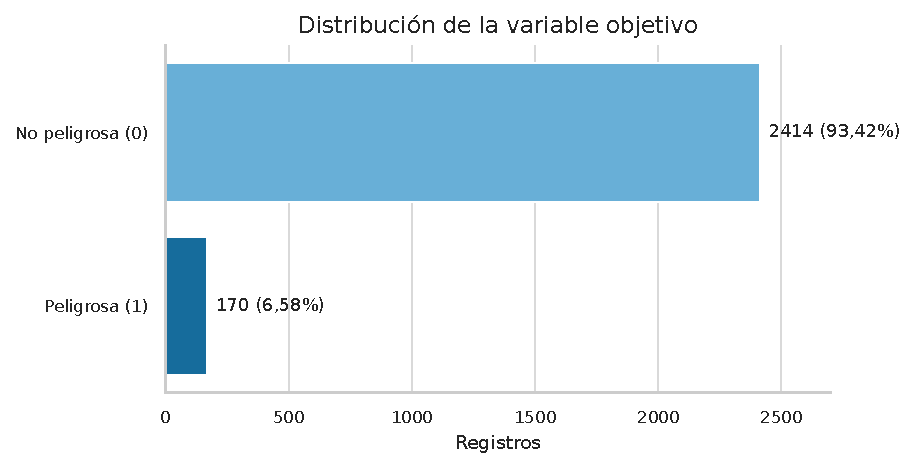
\includegraphics[width=0.72\textwidth]{output/figures/distribucion_clases.pdf}
\caption{Distribución de clases del conjunto \textit{Seismic-Bumps}.}
\label{fig:class-distribution}
\end{figure}

\subsection{Atributos predictivos documentados en el ARFF}
La Tabla~\ref{tab:attributes} resume los 18 atributos predictivos a partir del encabezado y las declaraciones \texttt{@attribute} del archivo ARFF. Cuando el ARFF declara un atributo como \texttt{real} pero no informa un rango mínimo y máximo, la tabla lo indica explícitamente. Esta decisión evita inventar rangos que no están respaldados por la fuente utilizada.

{\footnotesize
\setlength{\tabcolsep}{3pt}
\begin{longtable}{@{}p{0.18\textwidth}p{0.42\textwidth}p{0.14\textwidth}p{0.18\textwidth}@{}}
\caption{Atributos predictivos del conjunto \textit{Seismic-Bumps} según el ARFF.}\label{tab:attributes}\\
\toprule
\textbf{Atributo} & \textbf{Significado} & \textbf{Tipo} & \textbf{Valores posibles o rango} \\
\midrule
\endfirsthead
\toprule
\textbf{Atributo} & \textbf{Significado} & \textbf{Tipo} & \textbf{Valores posibles o rango} \\
\midrule
\endhead
\bottomrule
\endfoot
\texttt{seismic} & Resultado de la evaluación del peligro sísmico del turno en la labor minera mediante el método sísmico. & Nominal & \texttt{a,b,c,d}: sin peligro, bajo peligro, alto peligro, estado de peligro. \\
\texttt{seismoacoustic} & Resultado de la evaluación del peligro sísmico del turno mediante el método sismoacústico. & Nominal & \texttt{a,b,c,d}. \\
\texttt{shift} & Tipo de turno registrado. & Nominal & \texttt{W,N}: extracción de carbón o turno de preparación. \\
\texttt{genergy} & Energía sísmica registrada en el turno anterior por el geófono más activo. & Real & Rango no especificado en el ARFF. \\
\texttt{gpuls} & Número de pulsos registrados en el turno anterior por el geófono más activo. & Real & Rango no especificado en el ARFF. \\
\texttt{gdenergy} & Desviación de la energía registrada por el geófono más activo respecto de la energía promedio de los ocho turnos anteriores. & Real & Rango no especificado en el ARFF. \\
\texttt{gdpuls} & Desviación del número de pulsos registrado por el geófono más activo respecto del promedio de los ocho turnos anteriores. & Real & Rango no especificado en el ARFF. \\
\texttt{ghazard} & Evaluación del peligro sísmico obtenida por método sismoacústico usando solo el registro del geófono más activo. & Nominal & \texttt{a,b,c,d}. \\
\texttt{nbumps} & Número de eventos sísmicos registrados durante el turno anterior. & Real & Rango no especificado en el ARFF. \\
\texttt{nbumps2} & Número de eventos sísmicos del turno anterior en el intervalo de energía $[10^2,10^3)$. & Real & Rango no especificado en el ARFF. \\
\texttt{nbumps3} & Número de eventos sísmicos del turno anterior en el intervalo de energía $[10^3,10^4)$. & Real & Rango no especificado en el ARFF. \\
\texttt{nbumps4} & Número de eventos sísmicos del turno anterior en el intervalo de energía $[10^4,10^5)$. & Real & Rango no especificado en el ARFF. \\
\texttt{nbumps5} & Número de eventos sísmicos del último turno en el intervalo de energía $[10^5,10^6)$. & Real & Rango no especificado en el ARFF. \\
\texttt{nbumps6} & Número de eventos sísmicos del turno anterior en el intervalo de energía $[10^6,10^7)$. & Real & Rango no especificado en el ARFF. \\
\texttt{nbumps7} & Número de eventos sísmicos del turno anterior en el intervalo de energía $[10^7,10^8)$. & Real & Rango no especificado en el ARFF. \\
\texttt{nbumps89} & Número de eventos sísmicos del turno anterior en el intervalo de energía $[10^8,10^{10})$. & Real & Rango no especificado en el ARFF. \\
\texttt{energy} & Energía total de los eventos sísmicos registrados durante el turno anterior. & Real & Rango no especificado en el ARFF. \\
\texttt{maxenergy} & Energía máxima de los eventos sísmicos registrados durante el turno anterior. & Real & Rango no especificado en el ARFF. \\
\end{longtable}
}

La variable objetivo \texttt{class} no se cuenta como predictor. El ARFF define sus valores como \texttt{1} y \texttt{0}: el valor 1 indica que en el turno siguiente ocurrió un evento sísmico de energía mayor que $10^4$ J, mientras que el valor 0 indica que no ocurrió ese evento.

\subsection{Preparación de datos}
La preparación de datos se mantuvo deliberadamente simple y trazable. Se trabajó con un único archivo ARFF, \texttt{seismic-bumps.arff}, y no se integraron fuentes externas. El encabezado del archivo declara ausencia de valores faltantes; por lo tanto, no se aplicaron imputaciones ni eliminación de filas por datos incompletos.

Las variables nominales se conservaron como nominales según la declaración del ARFF. Las variables numéricas declaradas como \texttt{real} se trataron como variables cuantitativas. La normalización se aplicó solo donde corresponde por el algoritmo: se utilizó en k-NN porque el método depende de distancias y las escalas pueden alterar la noción de cercanía; no se aplicó al árbol de decisión porque este modelo no basa sus particiones en distancias entre instancias. En la regresión logística y en Naive Bayes se respetaron los flujos documentados en AI Studio y no se agregaron transformaciones no comprobadas.

SMOTE se aplicó únicamente en el subproceso de \textit{Training} de las variantes complementarias. El conjunto de \textit{Testing} conservó la distribución original y no recibió sobremuestreo. Esta decisión evita contaminación entre entrenamiento y prueba: los ejemplos sintéticos influyen en el ajuste del modelo, pero no modifican la evaluación.

No se realizó selección estadística de atributos. La decisión fue trabajar con los 18 predictores completos porque el objetivo del proyecto era comparar algoritmos bajo un procedimiento común y porque no se documentó una etapa validada de selección de variables dentro de los resultados disponibles. Introducir una selección posterior, sin incorporarla correctamente dentro de cada partición de la validación cruzada, habría creado una metodología diferente y potencialmente optimista. En consecuencia, el informe conserva el conjunto completo de predictores y declara esa decisión como parte del alcance.

\section{Metodología de evaluación}
Todos los resultados empíricos presentados provienen de Altair AI Studio mediante validación cruzada estratificada de 10 particiones. La estratificación busca conservar una proporción comparable de las dos clases en cada partición. En cada iteración, el modelo se entrena en el subconjunto de entrenamiento y se evalúa en el subconjunto de prueba correspondiente.

\begin{figure}[H]
\centering
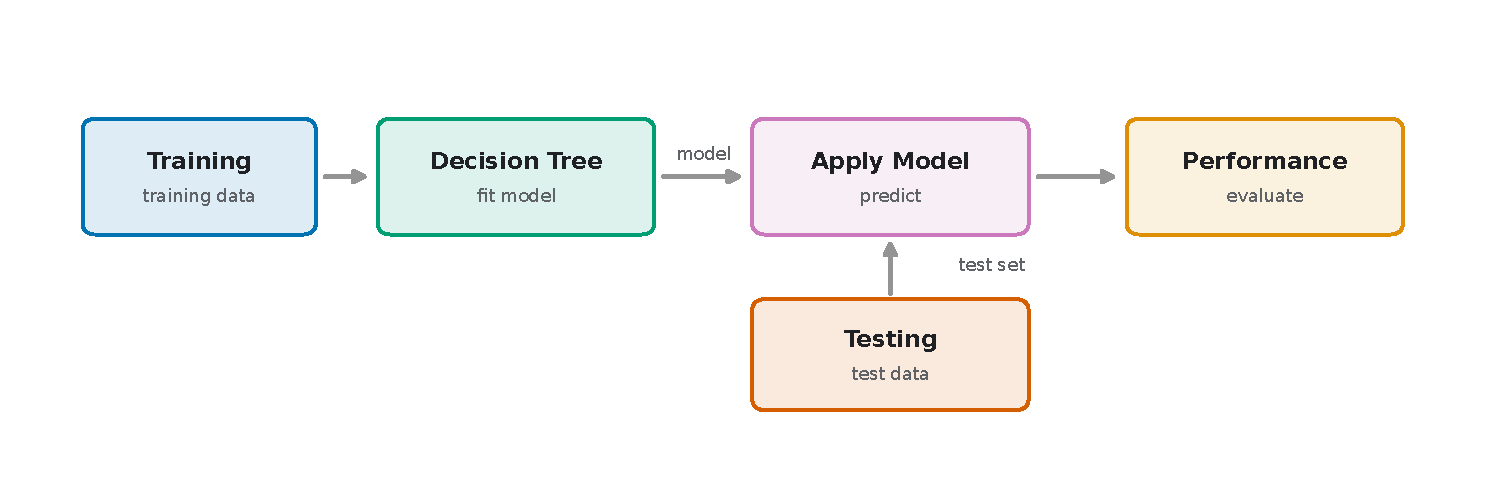
\includegraphics[width=0.86\textwidth]{output/figures/proceso_cross_validation_clean.pdf}
\caption{Esquema de la validación cruzada estratificada utilizada en la evaluación.}
\label{fig:cross-validation-process}
\end{figure}

Las matrices de confusión se presentan con filas verdaderas y columnas predichas. Con esta convención, para la clase peligrosa se define: verdadero positivo (TP) como un registro peligroso correctamente clasificado como peligroso; verdadero negativo (TN) como un registro no peligroso correctamente clasificado como no peligroso; falso positivo (FP) como un registro no peligroso clasificado como peligroso; y falso negativo (FN) como un registro peligroso clasificado como no peligroso. La precisión, el recall y el F1 de la clase 1 se calculan como:
\[
\mathrm{precision}=\frac{TP}{TP+FP},\qquad
\mathrm{recall}=\frac{TP}{TP+FN},
\]
\[
\mathrm{F1}=\frac{2\cdot\mathrm{precision}\cdot\mathrm{recall}}
{\mathrm{precision}+\mathrm{recall}}.
\]

Además de esas métricas, se reporta el AUC (optimistic) cuando AI Studio lo informó. La denominación se conserva tal como aparece en la herramienta y no se presenta como AUC estándar recalculado desde predicciones exportadas. Esta precisión metodológica es importante porque el informe no dispone de archivos de puntuaciones por instancia para reconstruir curvas ROC independientes.

\subsection{Algoritmos y parámetros documentados}
El árbol de decisión se usó como modelo interpretable basado en particiones sucesivas del espacio de atributos. Su propósito es separar las clases mediante reglas de decisión aprendidas a partir de los predictores. En los resultados disponibles se documenta el uso del operador \textit{Decision Tree} y una variante con SMOTE antes del learner; no se documentan hiperparámetros específicos adicionales, por lo que no se agregan valores no comprobados.

Naive Bayes se utilizó como clasificador probabilístico de referencia. Su propósito es estimar la clase más probable a partir de los atributos bajo el supuesto simplificador de independencia condicional. En el proyecto se documentan el modelo base y la variante con SMOTE aplicado en \textit{Training}; no se registran parámetros específicos adicionales en la evidencia disponible.

k-NN se evaluó como método basado en vecindad. Su propósito es clasificar cada instancia de acuerdo con las clases observadas en sus vecinos más cercanos. Como depende de distancias, se utilizó \textit{Normalize} antes del learner y se agrupó el preprocesamiento con el clasificador mediante \textit{Group Models}. El parámetro documentado es $k$, evaluado con los valores 3, 5, 7 y 9; para la comparación principal se conservó $k=5$ porque obtuvo el mayor recall y F1 de clase 1 entre esos candidatos.

La regresión logística se implementó mediante \textit{Generalized Linear Model} con familia binomial. Su propósito es estimar la probabilidad de pertenencia a la clase peligrosa mediante una función logística y convertir esa probabilidad en una predicción de clase según el umbral aplicado por la herramienta. Se documenta el uso de familia binomial y, en la variante complementaria, la aplicación de SMOTE antes de \textit{Generalized Linear Model}. No se agregan parámetros que no estén comprobados en la evidencia disponible.

\section{Resultados de los modelos base}
\subsection{Árbol de decisión}
El árbol de decisión base obtuvo una exactitud de 92,84\% $\pm$ 0,27\% y un AUC (optimistic) de 0,860 $\pm$ 0,041. La matriz de confusión muestra, sin embargo, que la exactitud se concentra casi por completo en la clase mayoritaria.

\begin{table}[H]
\centering
\caption{Matriz de confusión del árbol de decisión base.}
\label{tab:dt-base-matrix}
\begin{tabular}{lrr}
\toprule
& \textbf{Predicha 0} & \textbf{Predicha 1} \\
\midrule
\textbf{Verdadera 0} & 2394 & 20 \\
\textbf{Verdadera 1} & 165 & 5 \\
\bottomrule
\end{tabular}
\end{table}

La evidencia es clara: el modelo identifica correctamente 2394 registros no peligrosos, pero solo 5 de los 170 registros peligrosos. Esto produce 20 falsos positivos y 165 falsos negativos. A partir de la matriz acumulada, la precisión de la clase 1 es 20,00\%, el recall es 2,94\% y el F1 es 5,13\%. Por lo tanto, el árbol base no resulta adecuado cuando la prioridad es detectar la clase peligrosa.

\subsection{Naive Bayes}
Naive Bayes base obtuvo una exactitud de 84,75\% $\pm$ 4,31\% y un AUC (optimistic) de 0,761 $\pm$ 0,043. Su exactitud es menor que la del árbol, pero la matriz muestra una detección más alta de la clase 1.

\begin{table}[H]
\centering
\caption{Matriz de confusión de Naive Bayes base.}
\label{tab:nb-base-matrix}
\begin{tabular}{lrr}
\toprule
& \textbf{Predicha 0} & \textbf{Predicha 1} \\
\midrule
\textbf{Verdadera 0} & 2120 & 294 \\
\textbf{Verdadera 1} & 100 & 70 \\
\bottomrule
\end{tabular}
\end{table}

El modelo detecta 70 de los 170 casos peligrosos y deja 100 falsos negativos. El costo de esa mayor detección es un aumento de falsos positivos: 294 registros no peligrosos fueron clasificados como peligrosos. Las métricas agregadas son 19,23\% de precisión, 41,18\% de recall y 26,22\% de F1 para la clase 1. La interpretación es que Naive Bayes reduce omisiones respecto del árbol, pero genera más falsas alarmas.

\subsection{k-NN}
La evaluación de k-NN se realizó con normalización y con el preprocesamiento agrupado junto al clasificador. La Tabla~\ref{tab:knn-k-selection} resume la selección del parámetro $k$.

\begin{table}[H]
\centering
\caption{Selección del parámetro $k$ para k-NN.}
\label{tab:knn-k-selection}
\small
\begin{tabular}{@{}c c c c c c@{}}
\toprule
\textbf{$k$} & \textbf{Accuracy} & \shortstack{\textbf{AUC}\\\textbf{(optimistic)}} & \shortstack{\textbf{Precisión}\\\textbf{clase 1}} & \shortstack{\textbf{Recall}\\\textbf{clase 1}} & \shortstack{\textbf{F1}\\\textbf{clase 1}} \\
\midrule
3 & 92,38\% & 0,892 & 26,32\% & 8,82\% & 13,22\% \\
5 & 93,07\% & 0,851 & 39,02\% & 9,41\% & 15,17\% \\
7 & 93,23\% & 0,825 & 40,00\% & 5,88\% & 10,26\% \\
9 & 93,23\% & 0,804 & 36,84\% & 4,12\% & 7,41\% \\
\bottomrule
\end{tabular}
\end{table}

Entre los valores evaluados, $k=5$ obtuvo el mayor recall y el mayor F1 para la clase peligrosa. Su matriz acumulada fue:

\begin{table}[H]
\centering
\caption{Matriz de confusión de k-NN con $k=5$.}
\label{tab:knn-k5-matrix}
\begin{tabular}{lrr}
\toprule
 & \textbf{Predicha 0} & \textbf{Predicha 1} \\
\midrule
\textbf{Verdadera 0} & 2389 & 25 \\
\textbf{Verdadera 1} & 154 & 16 \\
\bottomrule
\end{tabular}
\end{table}

El modelo conserva una exactitud elevada, pero detecta solo 16 de los 170 registros peligrosos. La matriz produce 25 falsos positivos y 154 falsos negativos. En consecuencia, k-NN con $k=5$ mejora el árbol en detección de clase 1, pero sigue omitiendo la mayoría de los casos peligrosos.

\subsection{Regresión logística base}
La regresión logística base obtuvo una exactitud de 87,89\% $\pm$ 1,31\% y un AUC (optimistic) de 0,758 $\pm$ 0,051. Para la clase 1, AI Studio informó una precisión promedio de 25,69\% $\pm$ 3,64\%, un recall de 44,12\% $\pm$ 8,21\% y un F1 de 32,28\% $\pm$ 4,44\%.

\begin{table}[H]
\centering
\caption{Matriz de confusión de la regresión logística base.}
\label{tab:logistic-matrix}
\begin{tabular}{lrr}
\toprule
 & \textbf{Predicha 0} & \textbf{Predicha 1} \\
\midrule
\textbf{Verdadera 0} & 2196 & 218 \\
\textbf{Verdadera 1} & 95 & 75 \\
\bottomrule
\end{tabular}
\end{table}

A partir de los conteos acumulados, la precisión de clase 1 es 25,60\%, el recall es 44,12\% y el F1 es 32,40\%. Esta configuración detecta 75 casos peligrosos y deja 95 falsos negativos. La evidencia la ubica como la referencia más equilibrada entre los modelos base por F1 de clase 1, aunque no como la selección final si la prioridad principal es maximizar recall.

\begin{table}[H]
\centering
\caption{Comparación final de los cuatro modelos base.}
\label{tab:base-model-comparison}
\small
\resizebox{\textwidth}{!}{%
\begin{tabular}{@{}lccccc@{}}
\toprule
\textbf{Modelo} & \textbf{Exactitud} & \shortstack{\textbf{AUC}\\\textbf{(optimistic)}} & \shortstack{\textbf{Precisión agregada}\\\textbf{clase 1}} & \shortstack{\textbf{Recall agregado}\\\textbf{clase 1}} & \shortstack{\textbf{F1 agregado}\\\textbf{clase 1}} \\
\midrule
Árbol de decisión & 92,84\% $\pm$ 0,27\% & 0,860 $\pm$ 0,041 & 20,00\% & 2,94\% & 5,13\% \\
Naive Bayes & 84,75\% $\pm$ 4,31\% & 0,761 $\pm$ 0,043 & 19,23\% & 41,18\% & 26,22\% \\
k-NN ($k=5$) & 93,07\% & 0,851 & 39,02\% & 9,41\% & 15,17\% \\
Regresión logística & 87,89\% $\pm$ 1,31\% & 0,758 $\pm$ 0,051 & 25,60\% & 44,12\% & 32,40\% \\
\bottomrule
\end{tabular}%
}
\end{table}

\section{Experimento complementario con SMOTE}
SMOTE, propuesto por Chawla et al. (2002), se incorporó como tratamiento del desbalance en cuatro variantes: árbol de decisión, k-NN con $k=5$, regresión logística y Naive Bayes. En todos los casos, SMOTE se aplicó dentro de \textit{Training}, antes del algoritmo de aprendizaje, y \textit{Testing} permaneció con la distribución original. Esta metodología permite evaluar si el sobremuestreo mejora la detección de clase 1 sin contaminar el conjunto de prueba con ejemplos sintéticos.

\begin{figure}[H]
\centering
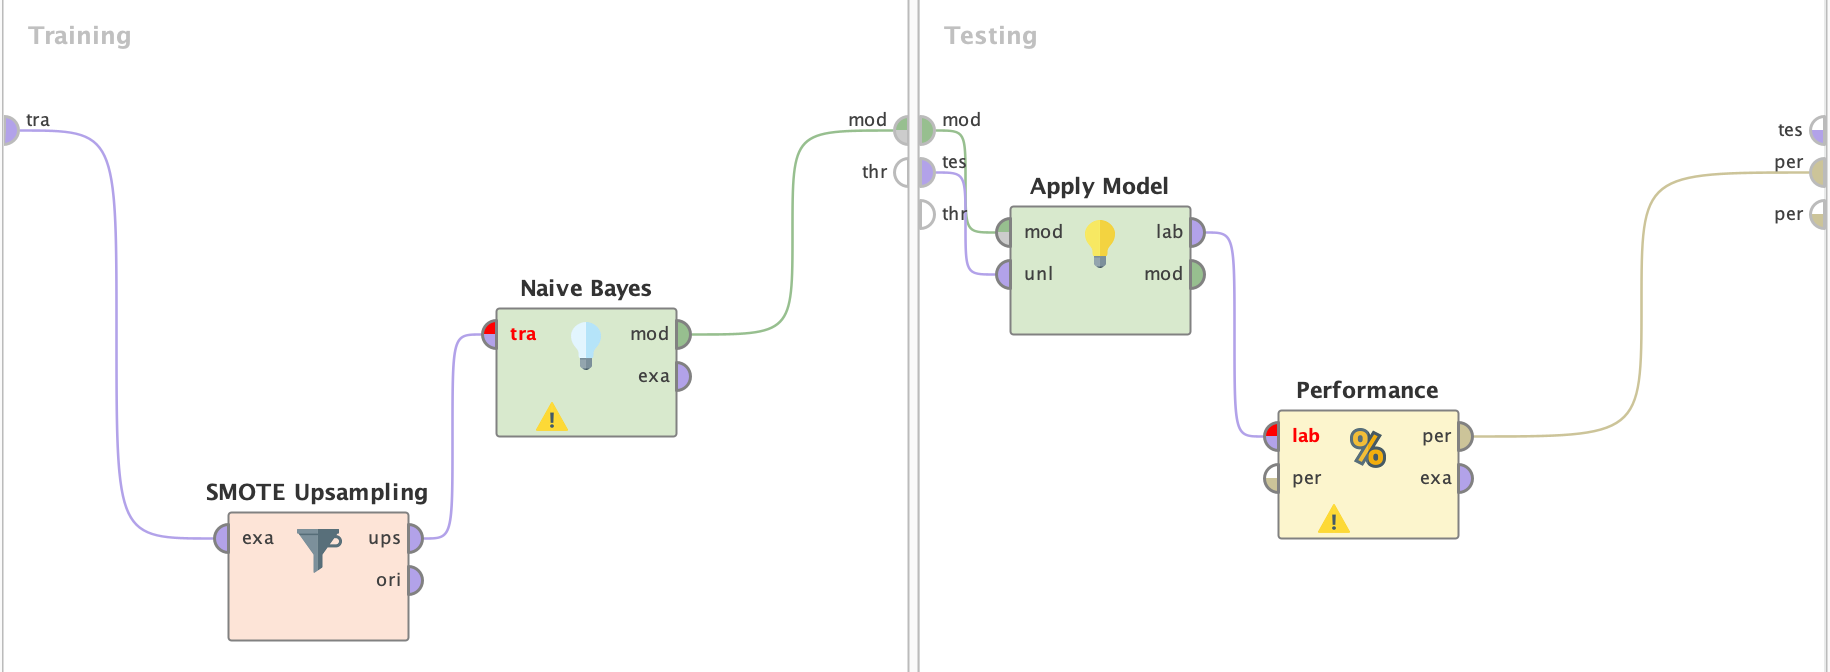
\includegraphics[width=0.96\textwidth]{output/figures/diagrama_smote_naive_bayes.png}
\caption{Flujo de Naive Bayes con SMOTE aplicado en \textit{Training}, seguido de \textit{Apply Model} y \textit{Performance}.}
\label{fig:smote-naive-bayes}
\end{figure}

La Tabla~\ref{tab:smote-variants-comparison} resume los resultados disponibles. La cuádrupla final de cada fila expresa TN / FP / FN / TP y mantiene la misma convención de matrices: filas verdaderas y columnas predichas.

\begin{table}[H]
\centering
\caption{Comparación de variantes verificadas con SMOTE.}
\label{tab:smote-variants-comparison}
\small
\resizebox{\textwidth}{!}{%
\begin{tabular}{@{}lcccccc@{}}
\toprule
\textbf{Variante} & \textbf{Exactitud} & \shortstack{\textbf{AUC}\\\textbf{(optimistic)}} & \shortstack{\textbf{Precisión}\\\textbf{clase 1}} & \shortstack{\textbf{Recall}\\\textbf{clase 1}} & \shortstack{\textbf{F1}\\\textbf{clase 1}} & \shortstack{\textbf{TN / FP / FN / TP}} \\
\midrule
Árbol de decisión & 80,77\% $\pm$ 4,33\% & 0,812 $\pm$ 0,065 & 18,62\% $\pm$ 3,74\% & 57,06\% $\pm$ 10,89\% & 28,08\% $\pm$ 5,21\% & 1990 / 424 / 73 / 97 \\
k-NN ($k=5$) & 79,68\% & 0,753 & 14,71\% & 43,53\% & 21,99\% & 1985 / 429 / 96 / 74 \\
Regresión logística & 51,63\% & 0,757 & 10,24\% & 81,76\% & 18,19\% & 1195 / 1219 / 31 / 139 \\
Naive Bayes & 69,93\% $\pm$ 17,58\% & 0,748 $\pm$ 0,034 & 13,65\% $\pm$ 3,58\% & 67,06\% $\pm$ 11,55\% & 22,69\% $\pm$ 5,08\% & 1693 / 721 / 56 / 114 \\
\bottomrule
\end{tabular}%
}
\end{table}

La evidencia muestra que SMOTE aumenta el recall de la clase peligrosa en todas las variantes, pero también incrementa los falsos positivos. Naive Bayes con SMOTE obtuvo 69,93\% de accuracy, AUC (optimistic) de 0,748, precisión de 13,65\%, recall de 67,06\% y F1 de 22,69\%. Su matriz contiene 1693 verdaderos negativos, 721 falsos positivos, 56 falsos negativos y 114 verdaderos positivos. En comparación con Naive Bayes base, detecta más casos peligrosos, pero reduce la precisión y aumenta las falsas alarmas.

La regresión logística con SMOTE representa el caso extremo de priorización del recall. Detecta 139 de los 170 casos peligrosos, por lo que deja 31 falsos negativos y alcanza 81,76\% de recall. La contracara es severa: clasifica como peligrosos 1219 registros no peligrosos y su precisión queda en 10,24\%. Por lo tanto, la mejora en cobertura es real, pero debe interpretarse como una decisión de costo: se aceptan muchas falsas alarmas para reducir omisiones peligrosas.

\section{Curvas ROC documentadas en AI Studio}
Las curvas ROC disponibles se incorporan como evidencia visual directa de AI Studio, no como una reconstrucción independiente. La Figura~\ref{fig:roc-smote-composite} reúne las cuatro capturas correspondientes a las variantes con SMOTE: Naive Bayes, regresión logística/Linear, k-NN con $k=5$ y árbol de decisión. En las capturas, la curva roja corresponde a ROC y la curva azul corresponde a los umbrales informados por la herramienta.

\begin{figure}[H]
\centering
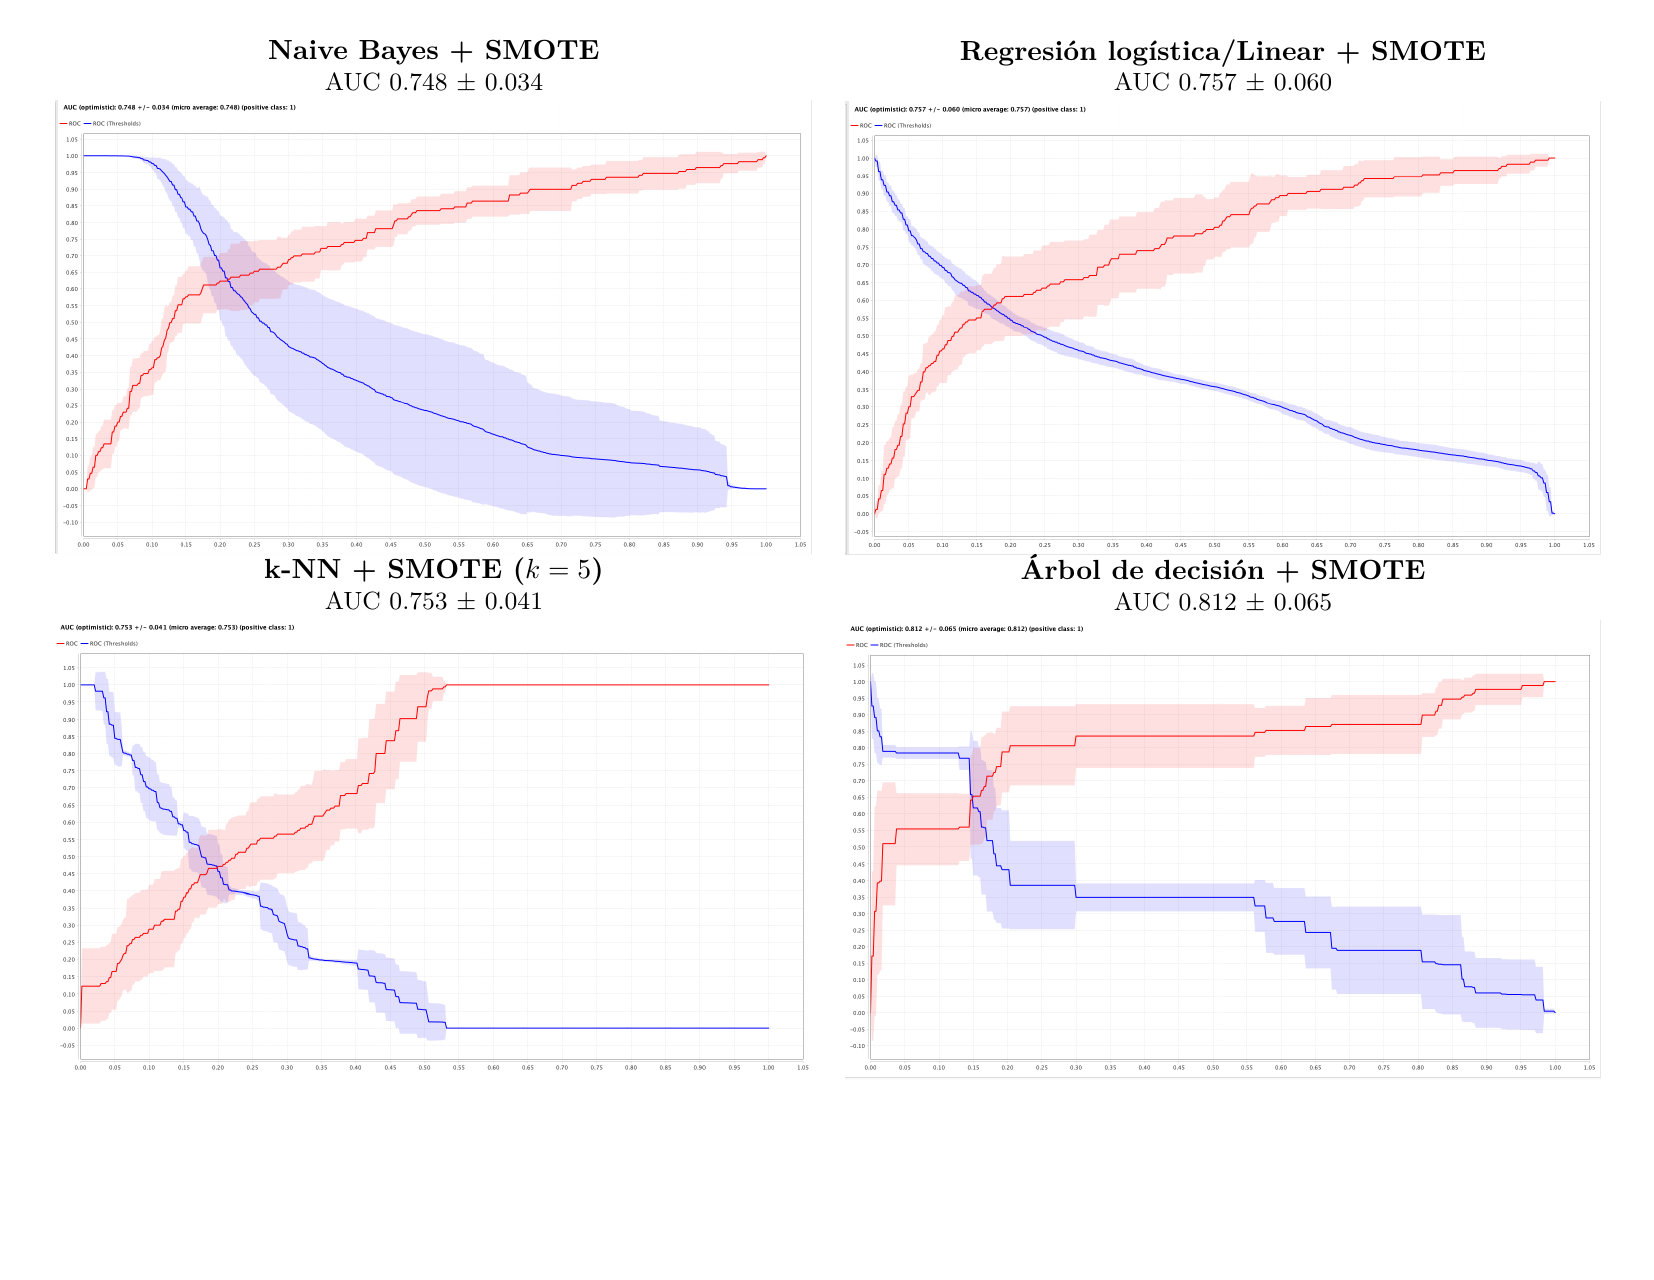
\includegraphics[width=0.88\textwidth]{output/figures/roc_smote_composite.png}
\caption{Capturas ROC de AI Studio para las variantes con SMOTE. La línea roja representa la curva ROC y la línea azul representa los umbrales. Los valores AUC mostrados son los reportados por AI Studio: Naive Bayes + SMOTE, 0,748 $\pm$ 0,034; regresión logística/Linear + SMOTE, 0,757 $\pm$ 0,060; k-NN + SMOTE con $k=5$, 0,753 $\pm$ 0,041; árbol de decisión + SMOTE, 0,812 $\pm$ 0,065.}
\label{fig:roc-smote-composite}
\end{figure}

La evidencia visual complementa las métricas agregadas de la Tabla~\ref{tab:smote-variants-comparison}. Sin embargo, su alcance es limitado: el informe no dispone de las probabilidades o puntuaciones por instancia de cada partición, por lo que no reconstruye curvas ROC fuera de AI Studio ni deriva puntos de umbral adicionales. Esta decisión preserva la trazabilidad metodológica y evita fabricar curvas a partir de AUC agregados.

\section{Análisis de error en función del número de atributos}
Este análisis es suplementario y corresponde a un proceso separado del experimento principal. Su objetivo fue explorar la sensibilidad de la tubería de regresión logística con SMOTE ante distintos números de atributos, sin reemplazar ni sobrescribir los resultados finales ya documentados para la regresión logística con SMOTE. En particular, la corrida con $k=18$ de este análisis de sensibilidad puede presentar una matriz de confusión ligeramente diferente a la corrida principal; por eso se interpreta como evidencia complementaria y no como nueva métrica final del modelo seleccionado.

En este proceso, los $k$ atributos superiores se seleccionaron mediante ganancia de información dentro de \textit{Training}. La evaluación usó validación cruzada estratificada de 10 particiones, y SMOTE se aplicó únicamente dentro de \textit{Training}; el subconjunto de \textit{Testing} conservó la distribución original. Esta organización evita contaminación entre entrenamiento y prueba y permite comparar el error medio de clasificación para distintos tamaños del subconjunto de atributos.

\begin{table}[H]
\centering
\caption{Error de clasificación de la regresión logística con SMOTE según número de atributos.}
\label{tab:error-atributos-logistica-smote}
\begin{tabular}{ccc}
\toprule
\textbf{Número de atributos} & \textbf{Error medio de clasificación} & \textbf{Variabilidad} \\
\midrule
3 & 39,09\% & $\pm$ 2,39\% \\
6 & 52,16\% & $\pm$ 14,04\% \\
9 & 50,46\% & $\pm$ 2,84\% \\
12 & 55,34\% & $\pm$ 3,94\% \\
15 & 49,31\% & $\pm$ 3,36\% \\
18 & 47,44\% & $\pm$ 5,64\% \\
\bottomrule
\end{tabular}
\end{table}

\begin{figure}[H]
\centering
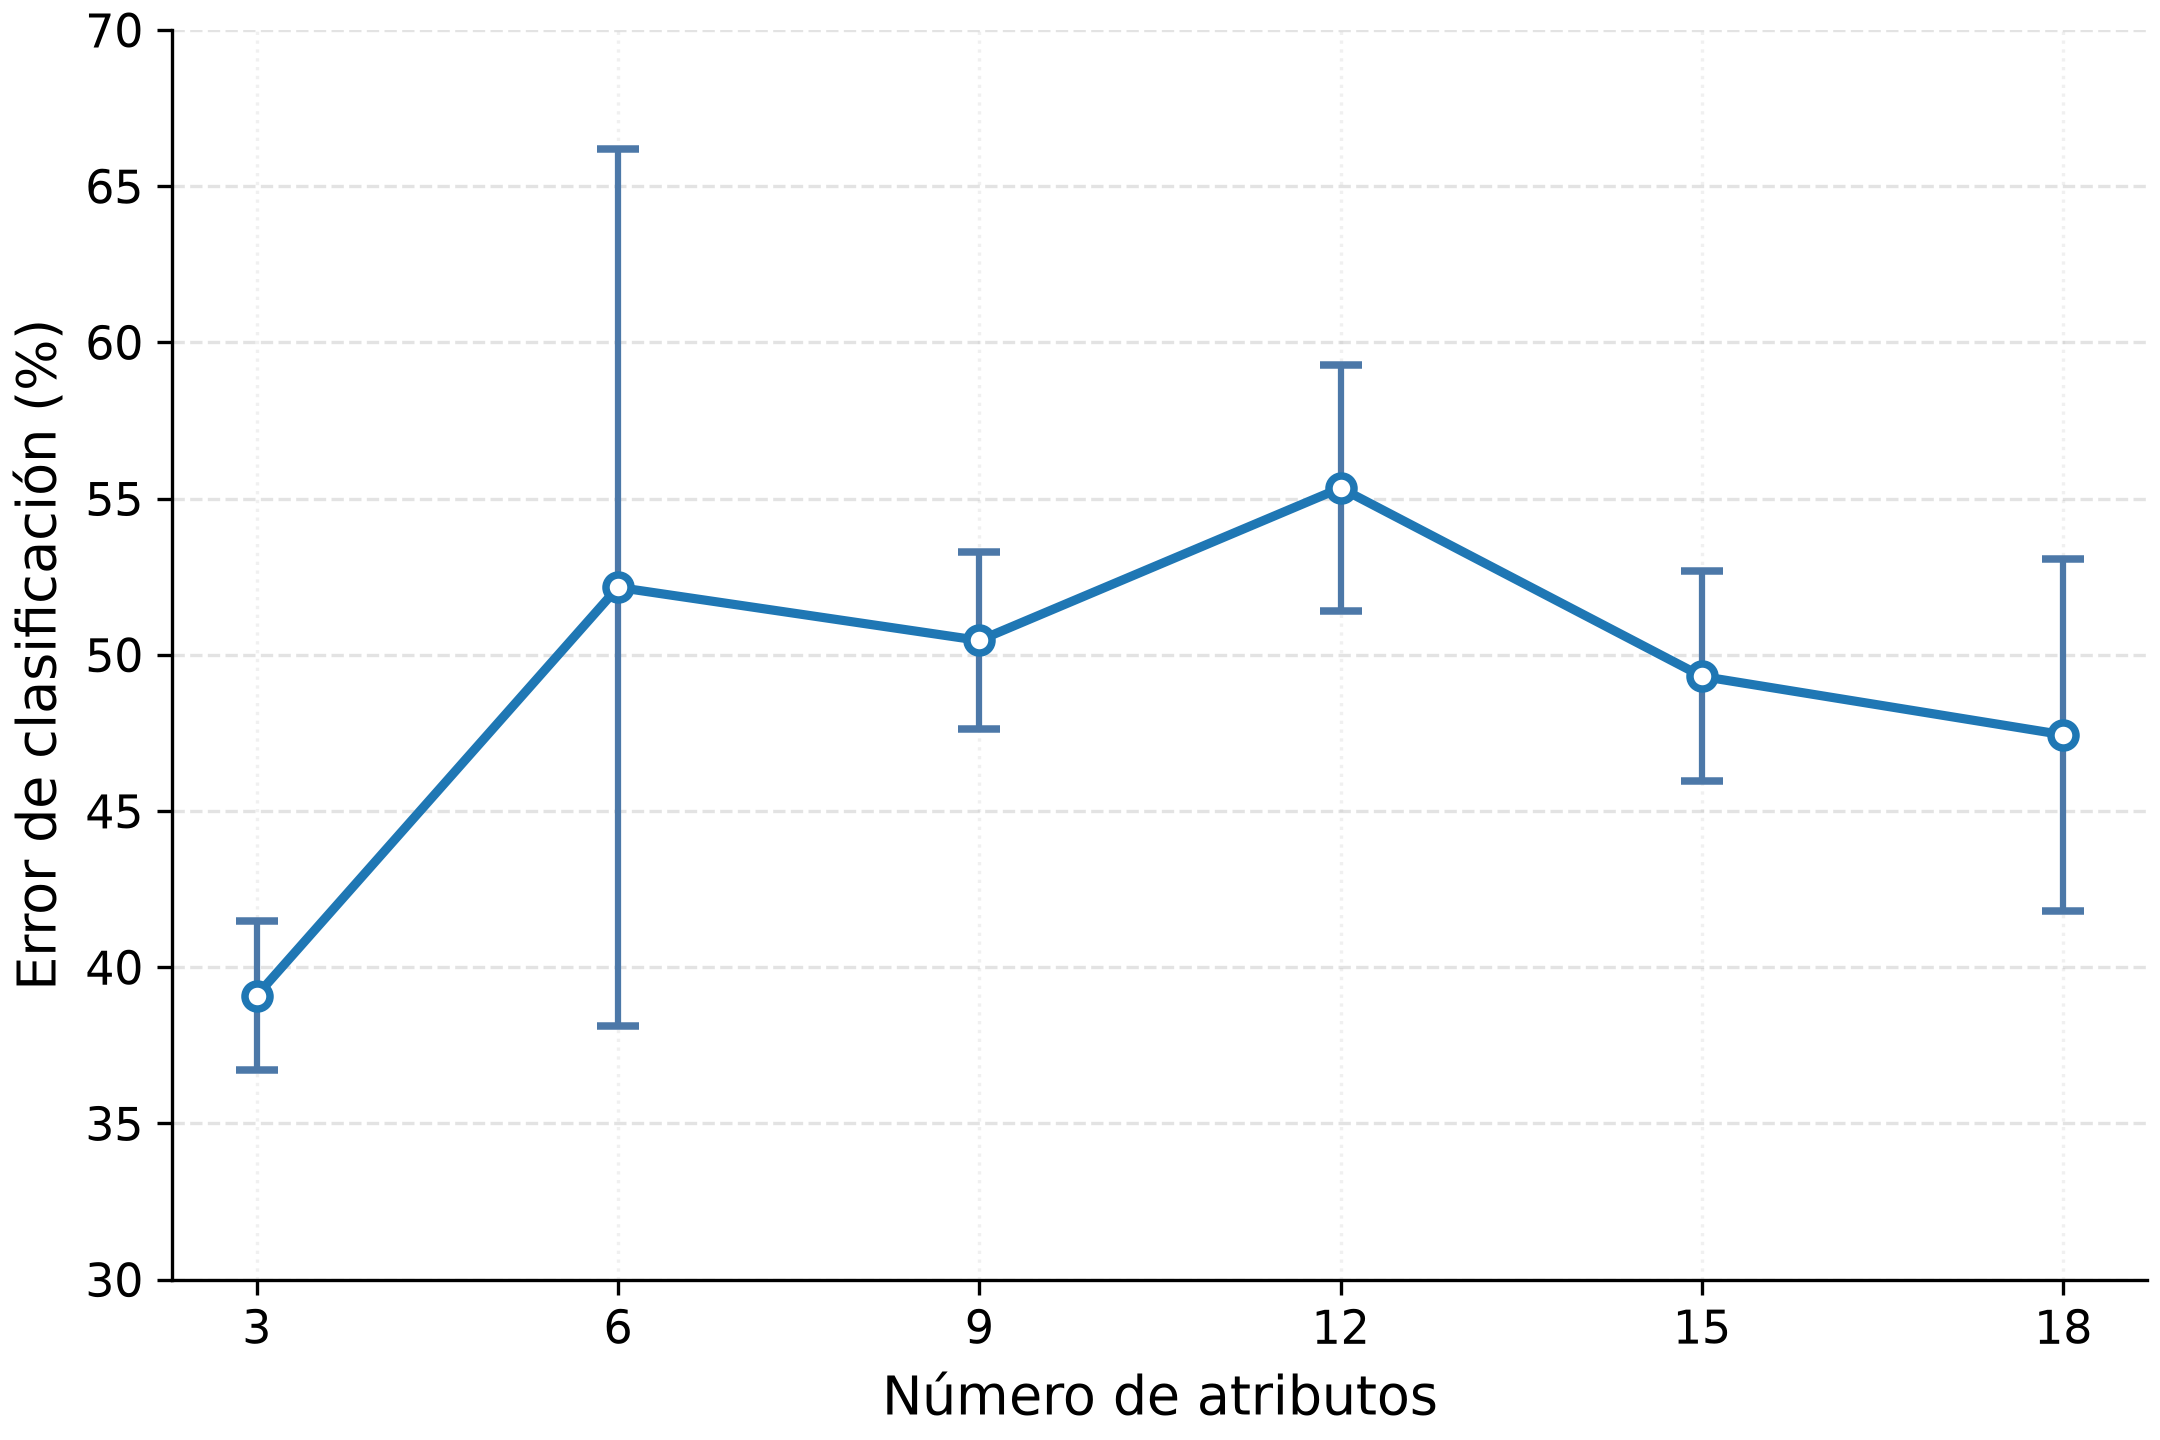
\includegraphics[width=0.86\textwidth]{output/figures/error_atributos_logistica_smote.png}
\caption{Error de clasificación de la tubería suplementaria de regresión logística con SMOTE en función del número de atributos seleccionados por ganancia de información dentro de \textit{Training}. Las barras de error representan la variabilidad reportada para cada validación cruzada estratificada de 10 particiones.}
\label{fig:error-atributos-logistica-smote}
\end{figure}

La evidencia no muestra una mejora monótona al aumentar el número de atributos. El menor error medio se observó con 3 atributos, mientras que 12 atributos produjo el mayor error medio reportado. No obstante, la variabilidad elevada en 6 atributos y el carácter suplementario del proceso impiden convertir este resultado en una nueva selección final. La interpretación prudente es que la selección de atributos puede modificar el comportamiento de la tubería, pero debería consolidarse en una experimentación específica antes de cambiar el modelo final del proyecto.

\section{Selección final del modelo}
La selección final debe responder al objetivo del proyecto, no a una preferencia abstracta por la métrica más alta. Si el objetivo es detectar la mayor proporción posible de casos peligrosos, el criterio principal es el recall de la clase 1 y la cantidad de falsos negativos. Bajo ese criterio, el modelo final seleccionado es \textbf{regresión logística con SMOTE}.

La evidencia que sostiene esta decisión es directa: regresión logística con SMOTE obtuvo 81,76\% de recall y redujo los falsos negativos a 31, el valor más bajo de todas las configuraciones evaluadas. Esto significa que detectó 139 de los 170 registros peligrosos. La interpretación es que esta configuración se alinea mejor con un objetivo preventivo, donde omitir un evento peligroso es el error más crítico.

La selección no oculta su costo. La misma variante produjo 1219 falsos positivos y una precisión baja de 10,24\%. En términos prácticos, eso implica muchas alertas sobre registros que en realidad pertenecen a la clase no peligrosa. Por lo tanto, la regresión logística con SMOTE no debe presentarse como un modelo globalmente superior, sino como la mejor opción dentro del criterio priorizado: maximizar la detección de la clase peligrosa.

La regresión logística base queda como referencia equilibrada por F1 entre los modelos base, con F1 agregado de 32,40\%, recall de 44,12\% y 95 falsos negativos. Esta referencia es útil para mostrar el intercambio entre equilibrio y cobertura. Sin embargo, no es la selección principal del proyecto, porque el criterio final prioriza recall de clase peligrosa por encima de F1.

\section{Discusión}
Los resultados confirman que la exactitud global es insuficiente para evaluar este problema. El árbol de decisión y k-NN alcanzan exactitudes superiores al 92\%, pero sus recalls de clase peligrosa son 2,94\% y 9,41\%, respectivamente. La evidencia indica que esos modelos clasifican muy bien la clase mayoritaria, pero fallan en el aspecto central del problema: detectar eventos peligrosos.

Naive Bayes y regresión logística base muestran una conducta menos conservadora. Naive Bayes detecta 70 casos peligrosos y la regresión logística base detecta 75. En ambos casos, el aumento del recall se paga con más falsos positivos que en k-NN o en el árbol. Esta diferencia permite interpretar el problema como una tensión entre falsas alarmas y omisiones. Si las falsas alarmas son muy costosas, puede preferirse un modelo más preciso; si la omisión de eventos peligrosos es más grave, resulta razonable priorizar recall.

SMOTE intensifica esa tensión. En todas las variantes aumenta la cobertura de clase 1 y reduce los falsos negativos, pero también disminuye la precisión. La regresión logística con SMOTE lleva esa lógica al máximo entre los resultados disponibles: alcanza el mayor recall, pero también la mayor cantidad de falsos positivos. Esta conducta no invalida la selección; la delimita. El modelo sirve para el objetivo preventivo definido, pero requiere una etapa posterior de calibración, umbral operativo y análisis de costos.

El proyecto, por lo tanto, no demuestra que exista una solución automática completa al problema de alerta sísmica. Demuestra algo más acotado y defendible: con los datos y la metodología disponibles, la regresión logística con SMOTE es la configuración que mejor reduce falsos negativos, mientras que la regresión logística base es la mejor referencia equilibrada por F1 entre los modelos base. Esa distinción evita una conclusión ambigua y permite separar evidencia, criterio de decisión y alcance operativo.

\section{Conclusiones}
El proyecto logró los objetivos planteados. Se describió el conjunto \textit{Seismic-Bumps}, se documentaron sus 18 atributos predictivos, se verificó la ausencia de faltantes declarada en el ARFF, se mantuvo una preparación de datos trazable y se compararon cuatro algoritmos bajo un procedimiento común de validación cruzada estratificada. También se incorporó el análisis de SMOTE sin contaminar \textit{Testing}, conservando la distribución original para evaluar los modelos.

Los resultados principales muestran que el desbalance domina la interpretación. El árbol de decisión base obtuvo 92,84\% de exactitud, pero solo 2,94\% de recall para la clase peligrosa. k-NN con $k=5$ alcanzó 93,07\% de exactitud y 9,41\% de recall. Naive Bayes base mejoró la detección con 41,18\% de recall, y la regresión logística base alcanzó el mejor F1 agregado entre modelos base, con 32,40\%. Con SMOTE, Naive Bayes obtuvo 69,93\% de accuracy, AUC (optimistic) de 0,748, precisión de 13,65\%, recall de 67,06\%, F1 de 22,69\% y matriz TN/FP/FN/TP de 1693/721/56/114.

La selección final única del proyecto es regresión logística con SMOTE. Se selecciona porque prioriza el recall de la clase peligrosa: obtuvo 81,76\% de recall y redujo los falsos negativos a 31. Esta conclusión es intencionalmente transparente sobre su costo: la variante produjo 1219 falsos positivos y una precisión baja de 10,24\%. En consecuencia, resuelve parcialmente el problema experimental de detección dentro del conjunto y la metodología utilizados, pero no resuelve por sí sola el problema operativo de alertas en minería.

Las oportunidades de mejora son claras. Primero, exportar predicciones y probabilidades por instancia para construir curvas ROC y análisis de umbral verificables. Segundo, validar con una partición temporal o con datos externos para evaluar generalización operativa. Tercero, incorporar un análisis explícito de costos entre falsos positivos y falsos negativos. Cuarto, profundizar la selección de atributos observada en el análisis suplementario, manteniendo esa selección dentro de \textit{Training} y separada de \textit{Testing} para evitar optimismo metodológico. Con esas extensiones, el proyecto podría pasar de una comparación experimental sólida a una propuesta de apoyo a la decisión más cercana al uso real.

\section{Referencias}
Chawla, N. V., Bowyer, K. W., Hall, L. O., \& Kegelmeyer, W. P. (2002). SMOTE: Synthetic Minority Over-sampling Technique. \textit{Journal of Artificial Intelligence Research, 16}, 321--357. \url{https://doi.org/10.1613/jair.953}

Sikora, M., \& Wrobel, L. (2010). Application of rule induction algorithms for analysis of data collected by seismic hazard monitoring systems in coal mines. \textit{Archives of Mining Sciences, 55}(1), 91--114.

Sikora, M., \& Wrobel, L. (s. f.). \textit{Seismic-Bumps} [Conjunto de datos]. UCI Machine Learning Repository. \url{https://archive.ics.uci.edu/dataset/266/seismic+bumps}

\end{document}
